
% !TEX encoding = UTF-8 Unicode 
% !TEX root = FieldGuide.tex

\Sec{Gamma Distribution}
\label{sec:Gamma}
\dist{Gamma} ($\Gamma$, Pearson type III)  distribution~\cite{Pearson1893, Pearson1895, Johnson1994} : 
%
\begin{align}
\label{Gamma}
\opr{Gamma}(x \given a, \theta, \alpha) 
&=  \frac{1}{\Gamma(\alpha)|\theta|} \left(\frac{x-a}{\theta}\right)^{\alpha-1} \exp\left\{-\frac{x-a}{\theta}\right\}  \checked
\\
\text{for } & x,\ a, \theta, \alpha \In  \mathbb{R}, \quad \alpha>0			
\notag												\checked
\\&=  \opr{Amoroso}(x\given  a, \theta, \alpha, 1) \notag 					\checked
\end{align}
The name of this distribution derives from the normalization constant.



\SSec{Special cases}
\phantomsection\addcontentsline{toc}{subsection}{~~~~~~~~~~~~Wein}
\phantomsection\addcontentsline{toc}{subsection}{~~~~~~~~~~~~Erlang}

Special cases of the beta prime distribution are listed in table~\ref{AmorosoTable}, under $\beta=1$.

The gamma distribution often appear as a solution to problems in statistical physics. For example, the energy density of a classical ideal gas, or the {\bf Wien} (Vienna) distribution $\op{Wien}(x\given T)=\opr{Gamma}(x\given 0, T,4)$, an approximation to the relative intensity of black body radiation as a function of the frequency. The {\bf Erlang} (m-Erlang) distribution~\cite{Erlang1909} is a gamma distribution with integer $\alpha$, which models the waiting time to observe $\alpha$ events from a Poisson process with rate $1/\theta$ ($\theta>0$). For $\alpha=1$ we obtain an exponential distribution \eqref{Exp}.


\begin{figure}[tp!]
\begin{center}
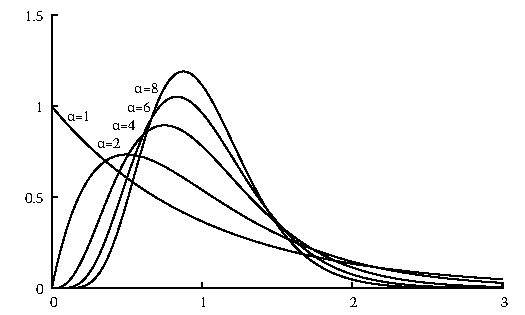
\includegraphics[width=\textwidth]{pdfGammaPDF}
\end{center}
\caption[Gamma distributions, unit variance]{Gamma distributions, unit variance $\opr{Gamma}(x\given \tfrac{1}{\alpha},\alpha)$}
\end{figure}



\dist{Standard gamma} (standard Amoroso) distribution~\cite{Johnson1994}: 
\[
\opr{StdGamma}(x\given \alpha) & = \frac{1}{\Gamma(\alpha)} x^{\alpha-1} e^{-x}		\checked
\label{StdGamma}
\\ & = \opr{Gamma}(x\given 0, 1, \alpha)
\]
    


\dist{Chi-square} ($\chi^2$)  distribution~\cite{Fisher1924,Johnson1994}:
\begin{align}
\label{ChiSqr}
\opr{ChiSqr}(x \given k) 
&= \frac{1}{2\Gamma(\tfrac{k}{2})} \left(\frac{x}{2}\right)^{\tfrac{k}{2}-1} 
\exp\left\{-\left(\frac{x}{2}\right)\right\} 	\checked
\\
& \qquad \text{for positive integer } k \notag \checked \\
&=  \opr{Gamma}(x\given  0, 2,\tfrac{k}{2}) \notag \checked \\
&=  \opr{Stacy}(x\given 2, \tfrac{k}{2},1) \notag \checked \\
&=  \opr{Amoroso}(x\given  0, 2, \tfrac{k}{2}, 1) \checked \notag 
\end{align}
The distribution of a sum of squares of $k$ independent standard normal random variables.  The chi-square distribution is important for statistical hypothesis testing in the frequentist approach to statistical inference.



\begin{figure}[t!]
\begin{center}
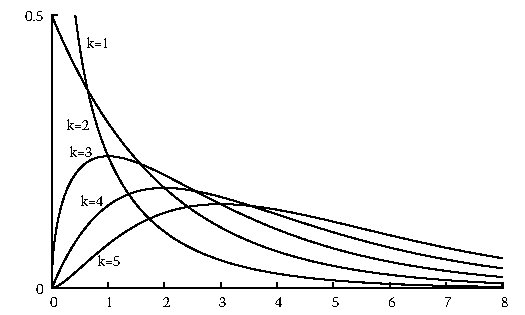
\includegraphics[width=\textwidth]{pdfChiSqr}
\end{center}
\caption[Chi-square distributions]{Chi-square distributions, $\opr{ChiSqr}(x\given k)$}
\end{figure}



\dist{Scaled chi-square}  distribution~\cite{Lee2012}:
\begin{align}
\label{ScaledChiSqr}
\opr{ScaledChiSqr}(x \given \sigma, k) 
&= \frac{1}{2\sigma^2\Gamma(\tfrac{k}{2})} \left(\frac{x}{2\sigma^2}\right)^{\tfrac{k}{2}-1} 
\exp\left\{-\left(\frac{x}{2\sigma^2} \right)\right\} \checked \\
& \qquad \text{for positive integer } k \notag \\
&=  \opr{Stacy}(x\given 2\sigma^2, \tfrac{k}{2},1)  \checked\notag \\
&=\opr{Gamma}(x\given 0, 2\sigma^2, \tfrac{k}{2}) \checked \notag \\
&=  \opr{Amoroso}(x\given  0, 2\sigma^2, \tfrac{k}{2}, 1) \checked \notag 
\end{align}
The distribution of a sum of squares of $k$ independent normal random variables with variance $\sigma^2$.


% !TEX encoding = UTF-8 Unicode 
% !TEX root = FieldGuide.tex

\begin{table*}[tp!]

\caption[Gamma distribution -- Properties]{Properties of the gamma distribution}

\begin{align*}
\text{\hyperref[PropertiesSec]{Properties}}  \quad& \\
\text{notation} \quad &  \op{Gamma}(x\given a, \theta, \alpha) 	\checked
\\
\text{PDF} \quad &
\frac{1}{\Gamma(\alpha)\Left|\theta\Right|} 
\Left(\frac{x-a}{\theta}\Right)^{\alpha  -1}
\exp \Left\{
-  \frac{x-a}{\theta}
\Right\}
\checked \hspace{-8em}						
\\ 
\text{CDF / CCDF } \quad  &    1-Q\Left(\alpha, \tfrac{x - a }{\theta} \Right) \checked
& \theta>0 \, \big/ \,  \theta<0
\\
\text{parameters}\quad &   a,\ \theta,\ \alpha,\  \text{in } \Real, \ \alpha>0
\\
\text{support} \quad &     x \geq a &  \theta > 0
\\
&   x\leq a  &  \theta < 0 
\\
%\text{median} \quad  &  \cdots
%\\
\text{mode} \quad&   a+ \theta (\alpha-1)
& \alpha   \geq 1 \checked
\\ & a & \alpha   \le 1 \checked
\\
\text{mean} \quad& a  + \theta \alpha \checked
\\
\text{variance}  \quad&   \theta^2 \alpha \checked & 
\\
\text{skew} \quad  &  \op{sgn}(\theta)\ \frac{2}{\sqrt{\alpha}}  \checked
\\
\text{ex. kurtosis} \quad  &  \frac{6}{\alpha} \checked
\\
\text{entropy} \quad& 
\ln \bigl(|\theta| \Gamma(\alpha) \bigr)+\alpha + \Left( 1 - \alpha\Right) \psi(\alpha) \checked
\\
\text{MGF} \quad  &   e^{a t} (1- \theta t)^{-\alpha}	\checked
% Wikipedia claims restriction that I don't immediately see in other texts.
\\
\text{CF} \quad  &  e^{i a t} (1- i \theta t)^{-\alpha}		\checked
\end{align*}
\end{table*}




\SSec{Interrelations}
\label{GammaInterrelations}



Gamma distributions with common scale obey an addition property:
\begin{align*}
\opr{Gamma}_1(0, \theta, \alpha_1) +  \opr{Gamma}_2(0, \theta,\alpha_2) \sim \opr{Gamma}_3(0, \theta,\alpha_1+\alpha_2)
\checked
\end{align*}
The  sum of two independent, gamma distributed random variables (with common $\theta$'s, but possibly different $\alpha$'s) is again a gamma random variable~\cite{Johnson1994}.

The Amoroso distribution can be obtained from the standard gamma distribution by the Weibull change of variables, $x \mapsto \left(\tfrac{x-a}{\theta}\right)^\beta$.
\[
\opr{Amoroso}(a ,\theta,\alpha,\beta) \sim
a+\theta \Big[{\opr{StdGamma}}(\alpha)\Big]^{1/\beta} 
\checked
\]


For large $\alpha$ the gamma distribution limits to normal~\eqref{Normal}.
\[
\opr{Normal}(x\given \mu,\sigma)   = 
\lim_{\alpha\rightarrow\infty} \opr{Gamma} (x\given  \mu- \sigma\sqrt{\alpha}, \tfrac{\sigma}{\sqrt{\alpha}}, \alpha)
\checked %Checked with MM
\]
Conversely, the sum of squares of normal distributions is a gamma distribution. See chi-square~\eqref{ChiSqr}.
\begin{align*}
\sum_{i=1,k}\oprr{StdNormal}{Normal}_i()^{2} & \sim \opr{ChiSqr}(k)  
 \sim \opr{Gamma}(0, 2,\frac{k}{2})  
 \checked
\end{align*}



A large variety of distributions can be obtained from transformations of 1~or~2 gamma distributions, which is convenient for generating pseudo-random numbers from those distributions (See appendix~\secref{sec:random}). \label{gammatransforms}
\begin{align*}
\opr{Normal}(\mu,\sigma)   &\sim  \mu+ \sigma\ \op{Sgn}()\ \sqrt{ 2 \opr{StdGamma}(\half) } 		& \eqref{Normal}
\checked
\\
\opr{GammaExp}(a,s,\alpha) &\sim a - s \ln\bigl(\opr{StdGamma}(\alpha)\bigr) 		& \eqref{GammaExp} \checked
\\
\opr{PearsonVII}(a,s, m) & \sim a + s\ \op{Sgn}() \sqrt{ \frac{(2m-1) \opr{StdGamma}_1(\half)}{\opr{StdGamma}_2(m-\half) } }		 \hspace{-1.5em}& \eqref{PearsonVII} 
% Devroye1986. 
\\
 \opr{Cauchy}(a,s) & \sim a + s\ \op{Sgn}() \sqrt{\frac{\opr{StdGamma}_1(\half)}{\opr{StdGamma}_2(\half) } } 		& \eqref{Cauchy} \checked % Devroye1986 p445
\\
\opr{UnitGamma}(a,s,\alpha,\beta) &\sim a+ s\ \exp  \bigl(- \tfrac{1}{\beta}\opr{StdGamma}(\alpha)\bigr)		& \eqref{UnitGamma} \checked
\\
%\opr{Beta}(a,s,\alpha,\gamma) & %& \eqref{Beta} \checked \\ \notag 
%\sim a + s\   \frac{\opr{StdGamma}_1(\alpha)}{\opr{StdGamma}_1(\alpha)+ \opr{StdGamma}_2(\gamma) }
%& \eqref{Beta} \checked 
%\\
\opr{Beta}(a,s,\alpha,\gamma) & 
\sim a + s\   \left(1 + \frac{\opr{StdGamma}_2(\gamma)}{\opr{StdGamma}_1(\alpha)} \right)^{-1}
& \eqref{Beta} \checked 
\\
\opr{BetaPrime}(a,s,\alpha,\gamma) &\sim  a + s\ \frac{\opr{StdGamma}_1(\alpha)}{\opr{StdGamma}_2(\gamma) }		& \eqref{BetaPrime}
\checked
\\
\opr{Amoroso}(a,\theta,\alpha,\beta)&\sim a + \theta\ \opr{StdGamma}(\alpha)^{\tfrac{1}{\beta}}		& \eqref{Amoroso}
\checked
\\
\opr{BetaExp}(a,s, \alpha,\gamma)  & 
\sim a - s\ \ln   \left(1 + \frac{\opr{StdGamma}_2(\gamma)}{\opr{StdGamma}_1(\alpha)} \right)^{-1}	
& \eqref{BetaExp} \checked  
\\
\opr{BetaLogistic}(a,s,\alpha,\gamma) &\sim  a - s \ln \left(\frac{\opr{StdGamma}_1(\alpha)}{\opr{StdGamma}_2(\gamma) } \right)		& \eqref{BetaLogistic} \checked
\\
\opr{GenBeta}(a,s,\alpha,\gamma,\beta) &
 \sim a + s  \left(1 + \frac{\opr{StdGamma}_2(\gamma)}{\opr{StdGamma}_1(\alpha)} \right)^{-\tfrac{1}{\beta}}		& \eqref{GenBeta} \checked
\\
\opr{GenBetaPrime}(a,s,\alpha,\gamma,\beta) & \sim  a+ s \left( \frac{\opr{StdGamma}_1(\alpha)}{\opr{StdGamma}_2(\gamma) }\right)^{\frac{1}{\beta}}		& \eqref{GenBetaPrime}
\checked 
\end{align*}
Here, $\op{Sgn}()$ is the sign (or Rademacher) discrete random variable: 50\% chance $-1$, 50\% chance $+1$.
\index{Rademacher distribution (discrete)|see{sign distribution}}
\index{sign distribution (discrete)}

